%\documentclass[10pt]{beamer}
%\usefonttheme[onlylarge]{structurebold}

\documentclass[handout]{beamer}
\usefonttheme[onlylarge]{structurebold}
  \usepackage{pgfpages}
\mode<handout>
\pgfpagesuselayout{4 on 1}[letterpaper,border shrink=5mm]

\hypersetup{
  bookmarks = false,
  colorlinks,
  citecolor = red,
  linkcolor=blue,
  urlcolor=blue,
  pdfpagemode=none,
  pdfstartview={Fit},
  pdftitle={},
  pdfauthor={Michael E. Waugh},
  pdfkeywords={} }
  \setbeamertemplate{navigation symbols}{}

\mode<presentation> {
  \usetheme{boxes}
  % or ...

  \setbeamercovered{transparent}
  % or whatever (possibly just delete it)
}

\setbeamertemplate{itemize subitem}[circle]
\setbeamerfont{frametitle}{size= \large}
\setbeamerfont{ framesubtitle }{size = \footnotesize}
\setbeamertemplate{frametitle}
{
\medskip
\smallskip
{\textsf{\underline{\insertframetitle\phantom{))))))))}}}}}


\usepackage[english]{babel}
\usepackage{wasysym}

\addfootbox{}{\hspace{4cm}\tiny {International Trade: Ricardian Model---Economics of Global Business, Revised: \today}}%

\title[NYU Stern] % (optional, use only with long paper titles)
{\Large International Trade: Ricardian Model}

\author[Michael Waugh] % (optional, use only with lots of authors)
{\bf{\Large}}%

\date[] % (optional)

\subject{Talks}

\begin{document}

\begin{frame}
  \titlepage
\end{frame}

%%%%%%%%%%%%%%%%%%%%%%%%%%%%%%%%%%%%%%%%%%%%%%%%%%%%%%%%%%%%%%%%%%%%%%%%%%%%%%%%%%%%%%%%%%%%%%%%%
%%%%%%%%%%%%%%%%%%%%%%%%%%%%%%%%%%%%%%%%%%%%%%%%%%%%%%%%%%%%%%%%%%%%%%%%%%%%%%%%%%%%%%%%%%%%%%%%%

\begin{frame}[t]
\frametitle{Recap\ldots}
\bigskip
\begin{itemize}
\item What we have done so far:
\begin{itemize}
\medskip
\item A country's opportunity cost,
\medskip
\item No trade relative prices,
\medskip
\item A country's PPF and no trade equilibrium.
\end{itemize}
\bigskip
\item Next\ldots
\begin{itemize}
\medskip
\item Pattern of trade (i.e. who will produce and export what),
\medskip
\item Prices at which countries are willing to trade internationally,
\medskip
\item Production, consumption, and gains from trade.
\medskip
\item Wages.
\end{itemize}
\end{itemize}
\end{frame}

%%%%%%%%%%%%%%%%%%%%%%%%%%%%%%%%%%%%%%%%%%%%%%%%%%%%%%%%%%%%%%%%%%%%%%%%%%%%%%%%%%%%%%%%%%%%%%%%%
%%%%%%%%%%%%%%%%%%%%%%%%%%%%%%%%%%%%%%%%%%%%%%%%%%%%%%%%%%%%%%%%%%%%%%%%%%%%%%%%%%%%%%%%%%%%%%%%%

\begin{frame}[t]
\frametitle{Comparative Advantage}
\bigskip
\begin{itemize}
\item Home opportunity cost
\begin{itemize}
\medskip
\item A wheat: 1/4$\times2 = 1/2$ cloth
\medskip
\item A cloth: 1/2$\times4 = 2$ wheat
\end{itemize}
\bigskip
\item Foreign opportunity cost
\begin{itemize}
\medskip
\item A wheat: 1/1$\times1 = 1$ cloth
\medskip
\item A cloth: 1/1$\times1 = 1$ wheat
\end{itemize}
\bigskip
\item Who has the comparative advantage?
\only<1>{\begin{itemize}
\medskip
\item The country with the lowest opportunity cost in a particular good has a comparative advantage in that good.
\end{itemize}
}
\only<2>{\begin{itemize}
\medskip
\item Wheat? Home gives up 1/2 cloth, Foreign gives up 1 cloth
\medskip
\item Cloth? Home gives up 2 wheat, Foreign gives up 1 wheat
\end{itemize}}
\end{itemize}
\bigskip
\end{frame}

%%%%%%%%%%%%%%%%%%%%%%%%%%%%%%%%%%%%%%%%%%%%%%%%%%%%%%%%%%%%%%%%%%%%%%%%%%%%%%%%%%%%%%%%%%%%%%%%%
%%%%%%%%%%%%%%%%%%%%%%%%%%%%%%%%%%%%%%%%%%%%%%%%%%%%%%%%%%%%%%%%%%%%%%%%%%%%%%%%%%%%%%%%%%%%%%%%%

\begin{frame}[t]
\frametitle{Comparative Advantage and Pattern of Trade}
\bigskip
\begin{itemize}
\item Comparative advantage dictates the pattern of trade
\begin{itemize}
\medskip
\item Home has a comparative advantage in wheat. It will want to produce and export wheat in return for cloth.
\medskip
\item Foreign has a comparative advantage in cloth. It will want to produce and export cloth in return for wheat.
\end{itemize}
\bigskip
\item At what prices will international trade occur\ldots
\begin{itemize}
\medskip
\item Note these prices must be consistent with voluntary exchange, i.e. where both countries are better off relative to no trade.
\end{itemize}
\end{itemize}
\end{frame}

%%%%%%%%%%%%%%%%%%%%%%%%%%%%%%%%%%%%%%%%%%%%%%%%%%%%%%%%%%%%%%%%%%%%%%%%%%%%%%%%%%%%%%%%%%%%%%%%%
%%%%%%%%%%%%%%%%%%%%%%%%%%%%%%%%%%%%%%%%%%%%%%%%%%%%%%%%%%%%%%%%%%%%%%%%%%%%%%%%%%%%%%%%%%%%%%%%%

\begin{frame}[t]
\frametitle{Relative Prices and Trade}
\bigskip
\begin{itemize}
\item From the perspective of the Home country:
\begin{itemize}
\medskip
\item If $P_w/P_c < 1/2$ will trade occur?
\bigskip
\item If $P_w/P_c > 1/2$ will trade occur?
\end{itemize}
\bigskip
\medskip
\item From the perspective of the Foreign country:
\begin{itemize}
\medskip
\item If $P_w/P_c < 1/1$ will trade occur?
\bigskip
\item If $P_w/P_c > 1/1$ will trade occur?
\end{itemize}
\only<2>{
\bigskip
\medskip
\item Only if $P_w/P_c$ lies in the interval $(1/2\ , \ 1)$ will trade occur between the Home and Foreign country.}
\end{itemize}
\end{frame}

%%%%%%%%%%%%%%%%%%%%%%%%%%%%%%%%%%%%%%%%%%%%%%%%%%%%%%%%%%%%%%%%%%%%%%%%%%%%%%%%%%%%%%%%%%%%%%%%%
%%%%%%%%%%%%%%%%%%%%%%%%%%%%%%%%%%%%%%%%%%%%%%%%%%%%%%%%%%%%%%%%%%%%%%%%%%%%%%%%%%%%%%%%%%%%%%%%%
\begin{frame}[t]
\frametitle{Recap}
\bigskip
\begin{itemize}
\medskip
\item Pattern of trade (i.e. who will produce and export what), $\Large {\color{red}\checkmark}$
\medskip
\item Prices at which countries trade, $\Large {\color{red}\checkmark}$
\medskip
\item Production, consumption, and gains from trade.
\medskip
\item Wages.
\end{itemize}
\bigskip
\bigskip
From here on out, we will assume the world price is $P^*_w/P^*_c = 2/3$.
\end{frame}

%%%%%%%%%%%%%%%%%%%%%%%%%%%%%%%%%%%%%%%%%%%%%%%%%%%%%%%%%%%%%%%%%%%%%%%%%%%%%%%%%%%%%%%%%%%%%%%%%
%%%%%%%%%%%%%%%%%%%%%%%%%%%%%%%%%%%%%%%%%%%%%%%%%%%%%%%%%%%%%%%%%%%%%%%%%%%%%%%%%%%%%%%%%%%%%%%%%

\begin{frame}[t]
\frametitle{Trade Equilibrium: Home Country}
\vspace{.2cm}
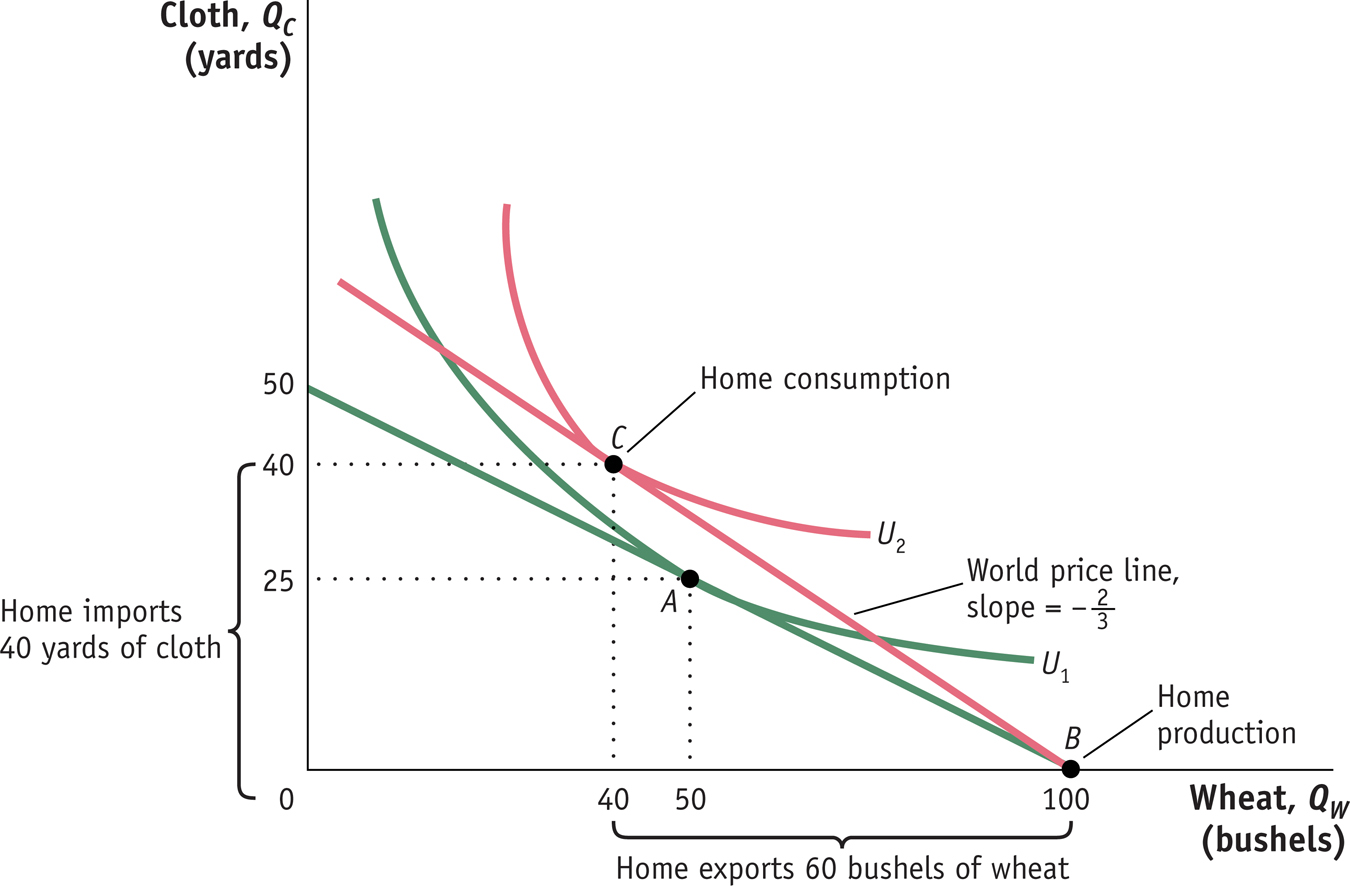
\includegraphics[height=3in,width=4.25in]{Feenstra_Essentials2e_fig_02_05.jpg}
\end{frame}

%%%%%%%%%%%%%%%%%%%%%%%%%%%%%%%%%%%%%%%%%%%%%%%%%%%%%%%%%%%%%%%%%%%%%%%%%%%%%%%%%%%%%%%%%%%%%%%%%
%%%%%%%%%%%%%%%%%%%%%%%%%%%%%%%%%%%%%%%%%%%%%%%%%%%%%%%%%%%%%%%%%%%%%%%%%%%%%%%%%%%%%%%%%%%%%%%%%

\begin{frame}[t]
\frametitle{Trade Equilibrium: Foreign Country}
\vspace{.2cm}
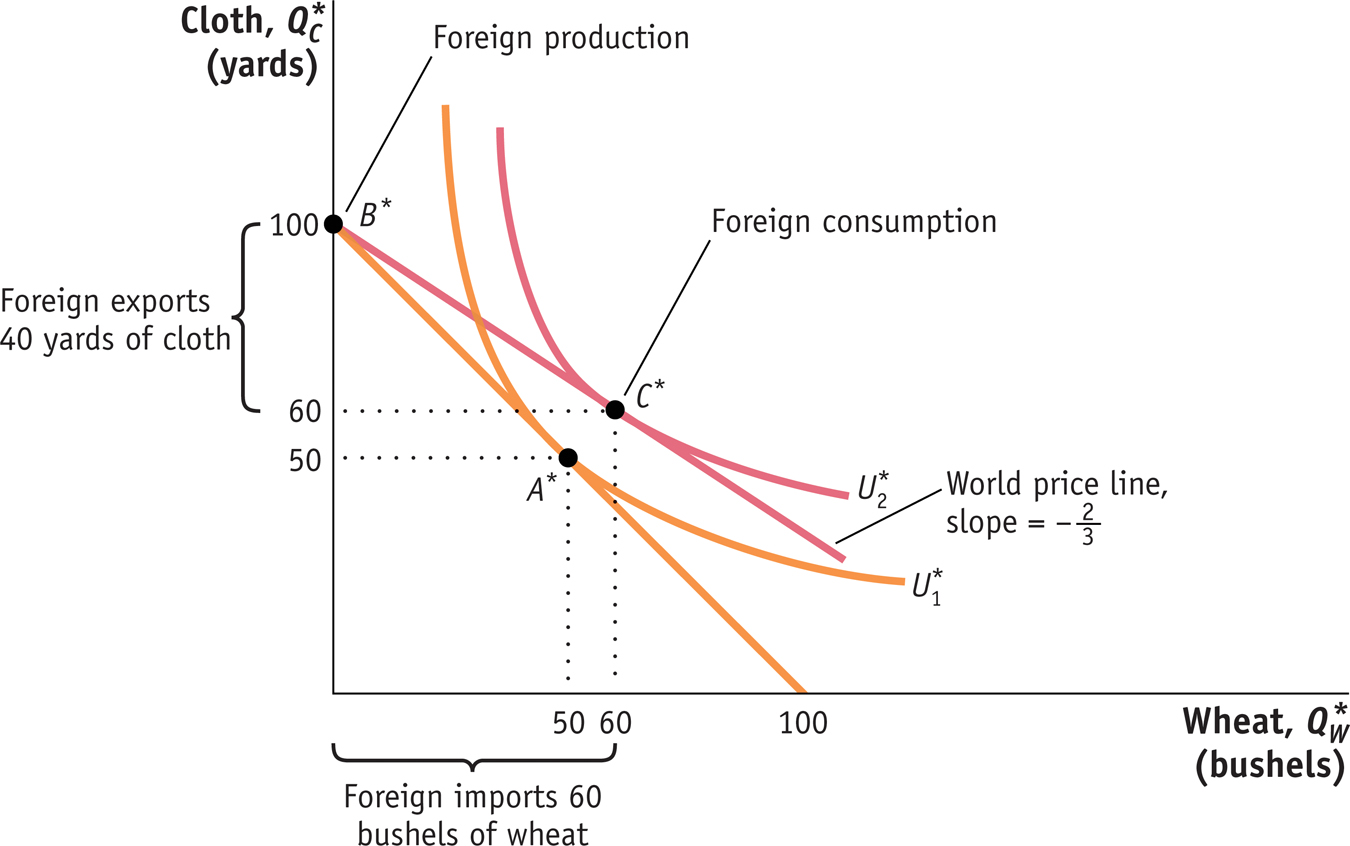
\includegraphics[height=3in,width=4.25in]{Feenstra_Essentials2e_fig_02_06.jpg}
\end{frame}

%%%%%%%%%%%%%%%%%%%%%%%%%%%%%%%%%%%%%%%%%%%%%%%%%%%%%%%%%%%%%%%%%%%%%%%%%%%%%%%%%%%%%%%%%%%%%%%%%
%%%%%%%%%%%%%%%%%%%%%%%%%%%%%%%%%%%%%%%%%%%%%%%%%%%%%%%%%%%%%%%%%%%%%%%%%%%%%%%%%%%%%%%%%%%%%%%%%

\begin{frame}[t]
\frametitle{Key Results}
\bigskip
\begin{itemize}
\item Comparative advantage shaped the pattern of production and trade.
\begin{itemize}
\medskip
\item Home specializes in wheat, Foreign specializes in cloth.
\end{itemize}
\bigskip
\item Consumers (in both countries) are strictly better off from trade. Two ways to see this\ldots
\begin{enumerate}
\medskip
\item In the figures, we locate at a higher indifference curve $U_2 > U_1$.
\medskip
\item Trade enlarges the consumption possibility set. If you have more choices, you must be better off.
\end{enumerate}
\end{itemize}
\end{frame}


%%%%%%%%%%%%%%%%%%%%%%%%%%%%%%%%%%%%%%%%%%%%%%%%%%%%%%%%%%%%%%%%%%%%%%%%%%%%%%%%%%%%%%%%%%%%%%%%%
%%%%%%%%%%%%%%%%%%%%%%%%%%%%%%%%%%%%%%%%%%%%%%%%%%%%%%%%%%%%%%%%%%%%%%%%%%%%%%%%%%%%%%%%%%%%%%%%%

\begin{frame}[t]
\frametitle{Home Wages}
\bigskip
\begin{itemize}
\item Note that because there are two goods, we need to pick the units to measure real wages. We will do both.
\bigskip
\item Home country real wages
\begin{itemize}
\medskip
\item In units of wheat $= MPL_w = $ 4
\medskip
\item In units of cloth $ = (P^*_w/P^*_c)\times MPL_w = $ 8/3
\bigskip
\item {\footnotesize Notice, with no trade, real wages were $4$ in units of wheat and $2$ in units of cloth. Independent of units, real wages are weakly higher from trade.}
\end{itemize}
\end{itemize}
\end{frame}


%%%%%%%%%%%%%%%%%%%%%%%%%%%%%%%%%%%%%%%%%%%%%%%%%%%%%%%%%%%%%%%%%%%%%%%%%%%%%%%%%%%%%%%%%%%%%%%%%
%%%%%%%%%%%%%%%%%%%%%%%%%%%%%%%%%%%%%%%%%%%%%%%%%%%%%%%%%%%%%%%%%%%%%%%%%%%%%%%%%%%%%%%%%%%%%%%%%

\begin{frame}[t]
\frametitle{Foreign Wages}
\bigskip
\begin{itemize}
\item Note that because there are two goods, we need to pick the units to measure real wages. We will do both.
\bigskip
\item Foreign country real wages
\begin{itemize}
\medskip
\item In units of wheat $= (P^*_c/P^*_w)\times  MPL_c = $ 3/2
\medskip
\item In units of cloth $ = MPL_c = $ 1
\bigskip
\item {\footnotesize Notice, with no trade, real wages were $1$ in units of wheat and $1$ in units of cloth. Independent of units, real wages are weakly higher from trade.}
\end{itemize}
\end{itemize}
\end{frame}

%%%%%%%%%%%%%%%%%%%%%%%%%%%%%%%%%%%%%%%%%%%%%%%%%%%%%%%%%%%%%%%%%%%%%%%%%%%%%%%%%%%%%%%%%%%%%%%%%
%%%%%%%%%%%%%%%%%%%%%%%%%%%%%%%%%%%%%%%%%%%%%%%%%%%%%%%%%%%%%%%%%%%%%%%%%%%%%%%%%%%%%%%%%%%%%%%%%

\begin{frame}[t]
\frametitle{Wages Summary}
\bigskip
\begin{itemize}
\item Home country real wages
\begin{itemize}
\medskip
\item In units of wheat $= MPL_w = $ 4
\medskip
\item In units of cloth $ = (P^*_w/P^*_c)\times MPL_w = $ 8/3
\end{itemize}
\bigskip
\item Foreign country real wages
\begin{itemize}
\medskip
\item In units of wheat $= (P^*_c/P^*_w) \times MPL_c = $ 3/2
\medskip
\item In units of cloth $ = MPL_c = $ 1
\end{itemize}
\bigskip
\item Home country real wages $>$ Foreign country real wages. Why?
\bigskip
\item The level of wages are determined by absolute advantage!
\end{itemize}
\end{frame}

%%%%%%%%%%%%%%%%%%%%%%%%%%%%%%%%%%%%%%%%%%%%%%%%%%%%%%%%%%%%%%%%%%%%%%%%%%%%%%%%%%%%%%%%%%%%%%%%%
%%%%%%%%%%%%%%%%%%%%%%%%%%%%%%%%%%%%%%%%%%%%%%%%%%%%%%%%%%%%%%%%%%%%%%%%%%%%%%%%%%%%%%%%%%%%%%%%%
\begin{frame}[t]
\frametitle{Recap}
\begin{itemize}
\item Pattern of trade (i.e. who will produce and export what)
\begin{itemize}
\medskip
\item Determined by comparative advantage.
\end{itemize}
\medskip
\item Prices at which countries trade
\begin{itemize}
\medskip
\item Must be such that both countries are willing to trade given their comparative advantage.
\end{itemize}
\medskip
\item Production, consumption, and gains from trade.
\begin{itemize}
\medskip
\item Production specializes according to comparative advantage. Consumptions possibilities enlarge leading to gains from trade.
\end{itemize}
\medskip
\item Wages.
\begin{itemize}
\medskip
\item Real wages increase for all. Absolute advantage determines the level of wages across countries.
\end{itemize}
\end{itemize}
\end{frame}

\end{document} 